\newpage
`
\newpage
\begin{appendices}
\section{Design Document} \label{App:design-document}

\subsection{  Content Based Access Control for Swift Storage }
Our proof of concept prototype works only on JSON formatted data stored in swift.

\subsubsection{ Usecase}
A data file ('data.json') is stored in swift. The owner of the file not only  specify who can or cannot access the file, but also define who can access how much content of the file, in other words,  she wants to specify access control on the content level of the file not only on the file level,  which essentially requires  finer grained access control than the existing Swift ACL. So, she  attaches a  policy ('policy.json')  with the file and wants that all the access request for the file would honor the policy associated with the file.

\subsubsection{Design Details}
We would attach a policy file with a file in the Swift storage. The policy file would specify who can or cannot access which part of the JSON document. The policy file would be stored as metadata associated with the file. In the object server, when we retrieve the file, we also retrieve the policy file. In our access control module we feed both the requested file and the policy file. The response from the access control module is the partial content of the file – the requester is allowed to access. Figure \ref{fig:swift-content-filter} shows the design diagram for our case.

\subsubsection{Proposed Changes}
The proposed changes are only at the object server middleware.

\begin{itemize}

\item \emph{Policy file}: We would specify syntax for policy file. The policy file would be stored as metadata associated with the file.
\item \emph{A/C Module}: The Access Control module takes a input file in JSON format and a policy file for it along with the credential of the requested user. The result from the A/C module is the partial content of the file – the requester is allowed to see.

\end{itemize}

\begin{figure*}[t]
\centering
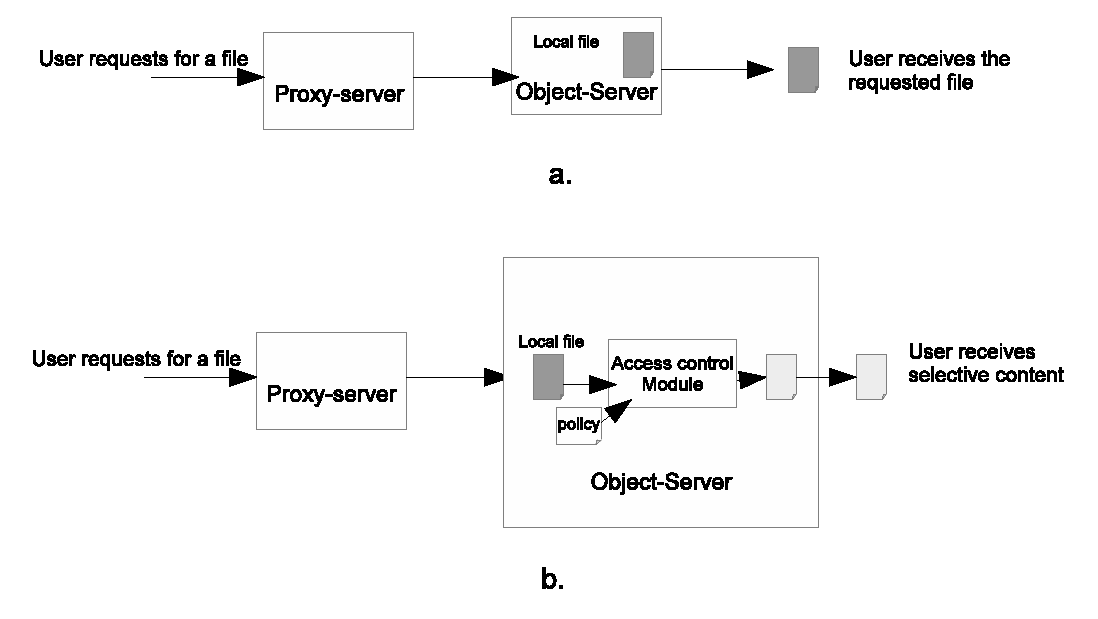
\includegraphics {eps/swift-content-filter}
\caption{a. Evaluation of GET Request for Swift, b.   Evaluation of GET Request for  Swift with Proposed Content Filter.}
\label{fig:swift-content-filter}
\end{figure*}

\subsection{ ZeroVM enabled Content Based Access Control for Swift Storage} 

\subsubsection{ Usecase}
ZeroVM enables a user to run arbitrary code on swift data inside swift storage by virtue of a ZeroVM Application. Assume a user now wants to run a ZeroVM application with an  arbitrary job, for example, a python script on a protected data file ('data.json'). With our proposed design, we would restrict any zerovm application to respect policy set by the owner of the swift data file.

This Use case differs from the former use case, in the sense that in the former case, a user is accessing a file, and in the later case, an application is accessing the file for purpose of further processing. While in the former case, there was no in Swift processing, in the later case user submitted untrusted code is to be executed. 

\subsubsection{Design Details} 
In the existing approach, in the manifest file of a ZeroVM application, user mentions input files, output files and image files (containing user application) and the launched ZeroVM inside the object server can access the full content of these files. In our proposed architecture, we let not allow full content of the input files to be visible to the user application. In order to achieve this, we introduce the concept of Query. In this case,  a manifest file contains a input file along with queries on that file.  In the final manifest for the ZeroVM, the input file is not given as a channel, rather the temporary files containing the output of the queries is used as channel. This is how, we would hide the visibility of the input file, and predetermined, controlled query result would be visible to the user ZeroVM Application. In processing the queries against the input file, we apply the policy associated with the  file. To make it simple, we use a JSONPath as the query language. While fig \ref{fig:abstracted-zapp} show the abstracted view of existing ZeroVM application, our proposed design detail is shown in fig \ref{fig:proposed-zapp}

\begin{figure*}[t]
\centering
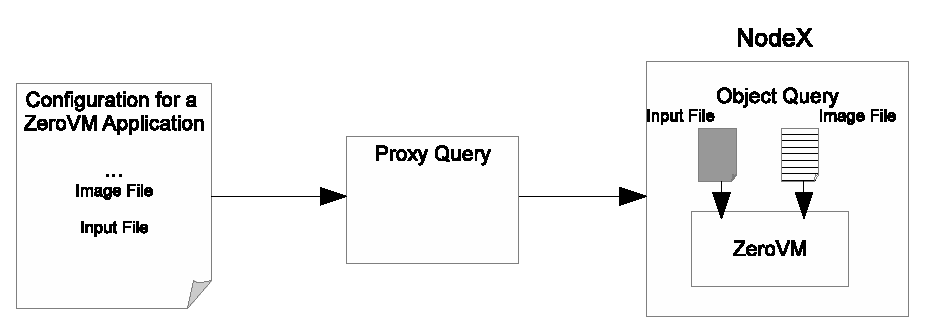
\includegraphics {eps/abstracted-zapp}
\caption{Abstracted Design for Existing ZeroVM Application .}
\label{fig:abstracted-zapp}
\end{figure*}

\begin{figure*}[t]
\centering
\includegraphics {eps/proposed-zapp}
\caption{Design for ZeroVM Application With Proposed Content Filter.}
\label{fig:proposed-zapp}
\end{figure*}

\subsubsection{Proposed Changes}
The proposed changes are made  at the manifest of the ZeroVM application along with at the object query middleware of the zerocloud.

\begin{itemize}

\item \emph{Add Query Section in the zapp Manifest}:  

\item \emph{Query Engine}: The query engine takes a query which is JSONPath in our case, and execute the query against the input files. The output of these queries are being saved in temporary files and these files are feed into the launched ZeroVM instead  of the original file.

\item \emph{A/C Module}: We develop an  access control module for JSON document which takes a JSON document, a policy file stating which part of the document is accessible by which user, and a set of queries. The module with the help of Query Engine generates output for these queries.

\end{itemize}

\end{appendices}
